%!TEX program = xelatex
\documentclass[12pt]{article}

% ---------- IDIOMA Y FUENTE ----------
\usepackage{fontspec} 
\usepackage[spanish, es-tabla, es-nodecimaldot]{babel} 
% --- Cambiar "Cuadro" por "Tabla" ---
\addto\captionsspanish{\renewcommand{\tablename}{Tabla}}
\setmainfont{TeX Gyre Termes}

% ---------- PAQUETES MATEMÁTICOS Y FÍSICOS ----------
\usepackage{amsmath,amssymb,amsfonts}
\usepackage{physics}

% ---------- GRÁFICOS Y COLORES ----------
\usepackage{xcolor}
\usepackage{subcaption}
\usepackage{graphicx}
\usepackage{tikz}
\usetikzlibrary{babel} 
\usepackage{tikz-3dplot}
\usetikzlibrary{shapes, arrows, positioning, calc}
\usetikzlibrary{arrows.meta} 
\usetikzlibrary{shapes.geometric} 
\usetikzlibrary{decorations.markings}

% ---------- CÓDIGO (LISTINGS) ----------
\usepackage{listings}
\definecolor{codegreen}{rgb}{0,0.6,0}
\definecolor{codegray}{rgb}{0.95,0.95,0.95}
\definecolor{codepurple}{rgb}{0.58,0,0.82}
\definecolor{backcolour}{rgb}{0.96,0.96,0.96}

\lstdefinestyle{pythonstyle}{
    backgroundcolor=\color{backcolour},   
    commentstyle=\color{codegreen},
    keywordstyle=\color{magenta},
    numberstyle=\tiny\color{gray},
    stringstyle=\color{codepurple},
    basicstyle=\ttfamily\small,          
    breakatwhitespace=false,         
    breaklines=true,                     
    captionpos=b,                    
    keepspaces=true,                 
    numbers=left,                        
    numbersep=5pt,                  
    showspaces=false,                
    showstringspaces=false,
    showtabs=false,                  
    tabsize=4,
    language=Python                      
}
\lstset{style=pythonstyle}

% ---------- DISEÑO Y ESTILO ----------
\usepackage{geometry}
\geometry{letterpaper, margin=2cm, headheight=15pt}
\usepackage{fancyhdr} 
\usepackage{lastpage}
\usepackage{wrapfig}
\usepackage{multicol}
\usepackage{enumitem}
\usepackage{framed}
\usepackage{etoolbox}

% ---------- TCOLORBOX ----------
\usepackage[most,skins,theorems]{tcolorbox}

% --- Caja para Definiciones Formales ---
\newtcolorbox{definicion}[1][]{
  enhanced,
  breakable, 
  colback=blue!5!white,
  colframe=blue!75!black,
  fonttitle=\bfseries,
  title={Definición: #1},
  arc=2mm,
  boxrule=0.8pt,
  drop shadow=black!10!white
}

% --- Caja para Tareas ---
\newtcolorbox{problemas}[1][]{
  enhanced,
  breakable, 
  colback=violet!6!white,       
  colframe=violet!45!white,     
  coltitle=violet!40!black,     
  fonttitle=\bfseries,
  title={Problemas: #1},
  arc=2.5mm,                    
  boxrule=0.8pt,
  drop shadow=black!8!white     
}

% --- Caja Libre Verde Menta ---
\newtcolorbox{cajaflex}[1][]{
  enhanced,
  breakable, 
  colback=teal!5!white,       
  colframe=teal!50!black,     
  coltitle=teal!10!white,     
  fonttitle=\bfseries,
  code={\ifblank{#1}{}{\tcbset{title={#1}}}},
  arc=2.5mm,                  
  boxrule=0.8pt,
  drop shadow=black!8!white   
}

% ---------- TABLAS Y ELEMENTOS EXTRA ----------
\usepackage{booktabs}   
\usepackage{pifont}     
\usepackage{array}      
\usepackage{caption}    
\newcommand{\lapiz}{\ding{46}\ }

% ---------- CONFIGURACIÓN DE ENCABEZADOS (ITM) ----------
\newcommand{\logo}{
\includegraphics[height=3cm]{escudoitm}}
\newcommand{\escola}{Facultad de Ciencias Exactas y Aplicadas}
\newcommand{\disc}{Física Computacional 1}
\newcommand{\auth}{Robinson Longas Bedoya}
\newcommand{\emaill}{\url{robinsonlongas@itm.edu.co}}
\newcommand{\email}{\url{robinsonlongas3586@correo.itm.edu.co}}
\newcommand{\cabec}{Física Computacional 1}

% ---------- ENLACES Y PDF ----------
\usepackage{hyperref}

\definecolor{myblue}{RGB}{20, 20, 120}
\definecolor{myred}{RGB}{220, 30, 30}
\definecolor{mygreen}{RGB}{0, 130, 60}

% Personalización de nombres para \autoref
\def\tableautorefname{Tabla}
\def\figureautorefname{Figura}
\def\equationautorefname{Ecuación}
\def\sectionautorefname{Sección}

\hypersetup{
    colorlinks=true,
    linkcolor=blue,
    urlcolor=blue,
    citecolor=blue,
    pdftitle={Física Computacional 1 -- Robinson Longas Bedoya},
    pdfauthor={Robinson Longas Bedoya}
}

% Configuración de estilos de página
\pagestyle{fancy}
\fancyhf{} 

\fancypagestyle{firstpage}{
    \fancyhead[L]{\logo}
    \fancyhead[R]{
        \textsf{\escola \\} 
        \textsf{\disc \\}
        \textsf{\auth \\}
        \textsf{\email \\} 
        \textsf{\emaill}     
    }
    \fancyfoot[R]{\scriptsize Página \thepage~de \pageref{LastPage}}
    \renewcommand{\headrulewidth}{0pt} 
    \renewcommand{\footrulewidth}{0.4pt} 
}

\fancyhead[L]{\textsf{\scriptsize \cabec\ -- \auth\ -- \email\ -- \emaill}}
\fancyfoot[R]{\scriptsize Página \thepage~de \pageref{LastPage}}
\renewcommand{\headrulewidth}{0.4pt} 
\renewcommand{\footrulewidth}{0.4pt} 

\setlength{\parskip}{0.3em}

\begin{document}
		\thispagestyle{firstpage}
		\vspace*{1.5cm}
	
	\begin{center}
		\rule{\textwidth}{0.4pt}
	\end{center}
	
	\begin{itemize}[leftmargin=*,label=\textcolor{red}{\ensuremath{\blacktriangleright}}]
		\item \textbf{Herramientas de Python para el cálculo:derivación e integración}
	\end{itemize}
	
	\noindent
	\textbf{\underline{Bibliografía}}
	\begin{itemize}[leftmargin=*, label={\textcolor{blue}{$\bullet$}}]
		\item \textit{Computational Physics}, Mark Newman.
      \item \textit{Programming for computations - Python}, Evein Linge and Petter Langtangen. 
      \item \textit{Computational Physics with Python}, Eric Ayars. 
      \item \textit{Computational mathematics: An introduction to Numerical Analysis and Scientific Computing  with Python},
      Dimitrios Mitsotakis. 
    \end{itemize}
     

\section*{\textcolor{red}{\textit{Derivación}}}

Recordemos,  desde la cinemática básica, si un cuerpo recorre 
una distancia de $\Delta x = 100\text{km}$ en un tiempo de 
$\Delta t = 2\text{ horas}$, su velocidad media es:
\begin{align*}
    v_{\text{prom}} = \frac{\Delta x}{\Delta t} = \frac{100\text{ km}}{2\text{ h}} = 50\text{ km/h}\,.
\end{align*}
Sin embargo, este valor no nos dice a qué velocidad avanzaba el vehículo en 
un instante exacto $t_0$. En realidad, 
el velocímetro marca distintos valores durante el trayecto.

Para medir el cambio instantáneo, reducimos el intervalo de tiempo 
$\Delta t$ haciéndolo cada vez más pequeño. La tasa de cambio en un
instante exacto corresponde al límite:
\begin{align*}
    v(t) = \lim_{\Delta t \to 0} \frac{x(t + \Delta t) - x(t)}{\Delta t} = \frac{dx}{dt}\,.
\end{align*}
Geométricamente, la derivada es la pendiente de la recta tangente 
a la curva en un punto específico.

Suponga que se dispone  de datos discretos 
(mediciones de tiempo $t$ y posición $x$). Usando la rutina 
 \texttt{np.gradient}, cuyo manual puede 
 \href{https://numpy.org/doc/stable/reference/generated/numpy.gradient.html}{cosultar aquí}
 podemos obtener la tasa de cambio instantánea en cada punto, veamos
%
\begin{lstlisting}[language=Python, captionpos=t, title=\texttt{derivada\_MRUA.py}]
import numpy as np

def x(t, x0=0., v0 = 0., a=2.5):
    'MRUA'
    return x0 + v0*t + 1/2. *a*t**2 

t = np.linspace(0,100,10)
x0 = float(input("Ingrese la posición inicial en m\n"))
v0 = float(input("Ingrese la velocidad inicial en m/s\n"))
a  = float(input("Ingrese la aceleración inicialen m0/s^2\n"))

r = x(t,x0,v0,a)

# velocidad v(t) = dx/dt
v_num = np.gradient(r, t)
# aceleración a(t) = dv/dt 
a_num = np.gradient(v_num, t)


v_num2 = np.gradient(r, t, edge_order=2)
a_num2 = np.gradient(v_num2, t, edge_order=2)

# velocidad analítica v(t) = v0 + a * t 
v_exacta = v0 + a*t
# aceleración analítica a(t) = a 
a_exacta = a    

print("\n" + "="*50)
print("Velocidad exacta:    \n", np.round(v_exacta, 2))
print("Velocidad numérica:  \n", np.round(v_num, 2))
print("-" * 50)
print("Aceleración exacta:  \n", a_exacta)
print("Aceleración numérica:\n", np.round(a_num, 2))
print("="*50)
print("Velocidad numérica edge_order2:  \n", np.round(v_num2, 2))
print("-" * 50)
print("Aceleración numérica edge_order2:\n", np.round(a_num2, 2))
print("="*50)
\end{lstlisting}
%  
Cuando se trabaja con funciones en papel, la derivada se define 
mediante un límite infinitesimal. Sin embargo, numéricamente se trabaja con 
\textbf{muestras discretas} 
(mediciones tomadas a intervalos de tiempo $\Delta t$ o espacio $\Delta x$).
La función \texttt{np.gradient()} de NumPy nos permite calcular la tasa de 
cambio instantánea (derivada numérica) a lo largo de un arreglo 
de datos utilizando el método de \textbf{diferencias finitas} (este lo 
estudiaremos en detalle en la continuación de este curso). El algoritmo calcula 
la derivada tomando el cuenta los vecinos hacia adelante y haci atrás. En los extremos,
no se tienen vecinos y pr eso los valores numéricos no coinciden con los análiticos.
Note que con el argumento \lstinline|edge_order =2| corregimos el error.

\subsection*{\textcolor{blue}{\textit{Ejemplo: la derivada de $\sin(x)$}}} 
%
\begin{lstlisting}[language=Python, captionpos=t, title=\texttt{derivada\_sinx.py}]
import numpy as np
import matplotlib.pyplot as plt

N =  50 # número de úntos
x = np.linspace(0,2*np.pi,N)

y = np.sin(x) 

dy = np.cos(x) # derivada exacta de sin(x)

# derivadas numéricas
dy1 =  np.gradient(y, x, edge_order=1) 
dy2 =  np.gradient(y, x, edge_order=2)

#errores
error1 = np.abs(dy - dy1)
error2 = np.abs(dy - dy2)

#plots
fig, (ax1, ax2) = plt.subplots(2, 1, figsize=(10, 10), sharex=True)

# Subplot 1: Función y derivadas
ax1.plot(x, y, "k--", alpha=0.5, lw = 2,label=r"$f(x) = \sin(x)$")
ax1.plot(x, dy, "k-", lw=2, label=r"Analítica: $\cos(x)$")
ax1.plot(x, dy1, "ro", markersize=5, label=r"Numérica (edge_order=1)")
ax1.plot(x, dy2, "b.", markersize=4, label=r"Numérica (edge_order=2)")
ax1.grid(True, ls=":", alpha=0.6)
ax1.legend(loc="lower left")

# Subplot 2: Error absoluto
ax2.semilogy(x, error1, "r-o", markersize=4, label=r"Error $|f'_{exacta} - f'_{num}|$ (edge=1)")
ax2.semilogy(x, error2, "b-s", markersize=4, label=r"Error $|f'_{exacta} - f'_{num}|$ (edge=2)")
ax2.set_xlabel(r"$x$ (rad)", fontsize=11)
ax2.set_ylabel("Error absoluto", fontsize=11)
ax2.grid(True, which="both", ls=":", alpha=0.6)
ax2.legend(loc="lower center")

plt.tight_layout()
#plt.savefig('../Clases/Herramientas_Python/derivadasinx.pdf', bbox_inches='tight')
plt.show()
\end{lstlisting}
%

%
\begin{figure}[htbp]
    \centering
    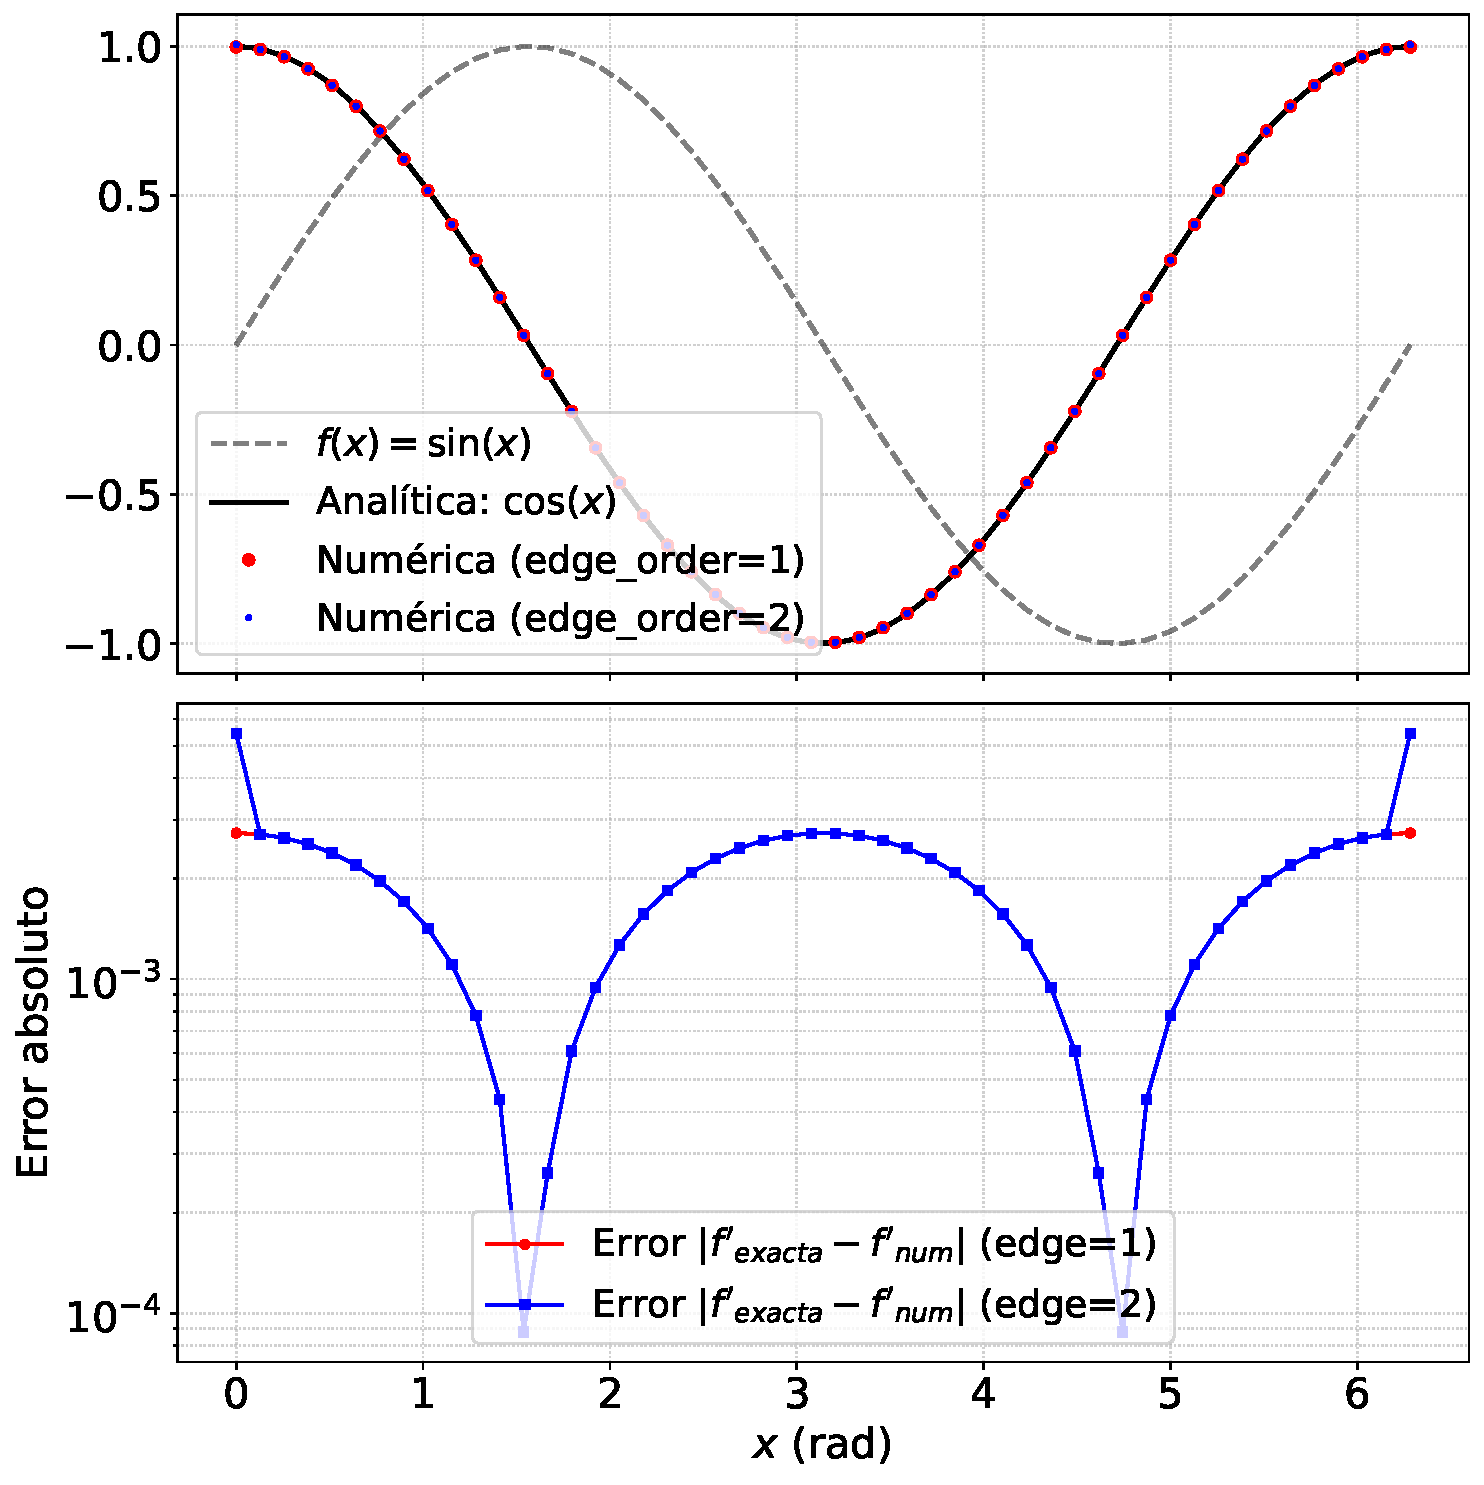
\includegraphics[width=0.5\textwidth]{derivadasinx.pdf}
    \caption{Derivada numérica de $f(x)  = \sin (x)$.}
\end{figure}
%

\newpage 
\begin{cajaflex}[ Resumen del uso de \texttt{numpy.gradient}]

$\blacklozenge$ Acceda a la documentación oficial \lstinline|scipy.optimize.root_scalar| 
\href{https://numpy.org/doc/stable/reference/generated/numpy.gradient.html}{dando clic aquí}.

\lstinline|numpy.gradient(f, *varargs, axis=None, edge_order=1)|

\textcolor{teal!60!black}{\rule{\linewidth}{0.8pt}}

\vspace{0.1cm}

\subsubsection*{\textcolor{teal!70!black}{1. \texttt{f} \mdseries{(Obligatorio)}}}
\begin{itemize}
    \item El arreglo de datos (\textit{1D, 2D o N-dimensional}) al que se le quiere calcular la derivada.
\end{itemize}

\subsubsection*{\textcolor{teal!70!black}{2. \texttt{*varargs} \mdseries{(Opcional)}}}
\begin{itemize}
    \item La variable independiente respecto a la que se deriva.
    \item \textbf{Formas de especificarlo:}
    \begin{itemize}
        \item \textbf{Sin argumento:} Asume un espaciado unitario ($\Delta x = 1$).
        \item \textbf{Un número escalar (\texttt{dx = 0.1}):} Indica que la distancia constante entre cada punto es $0.1$.
        \item \textbf{Un vector (\texttt{t}):} Pasa el arreglo de coordenadas exactas. Es la opción ideal si los puntos no están espaciados de forma uniforme.
    \end{itemize}
\end{itemize}

\subsubsection*{\textcolor{teal!70!black}{3. \texttt{axis} \mdseries{(Opcional, por defecto \texttt{None})}}}
\begin{itemize}
    \item Dirección o eje a lo largo del cual se deriva cuando se trabaja con matrices o arreglos multidimensionales.
    \item \textbf{Comportamiento:}
    \begin{itemize}
        \item \textbf{En vectores 1D:} Se ignora o se deja por defecto.
        \item \textbf{En matrices 2D:} \texttt{axis=None} calcula el gradiente en filas y columnas. \texttt{axis=0} deriva solo verticalmente; \texttt{axis=1} deriva solo horizontalmente.
    \end{itemize}
\end{itemize}

\subsubsection*{\textcolor{teal!70!black}{4. \texttt{edge\_order} \mdseries{(Opcional, por defecto \texttt{1})}}}
\begin{itemize}
    \item Es el nivel de precisión empleado para evaluar la derivada \textbf{únicamente en los bordes} (primer y último punto).
    \item \textbf{Opciones:}
    \begin{itemize}
        \item \textbf{\texttt{1}:} Usa $2$ puntos para trazar una recta en el borde. 
        Eficiente, pero introduce error en los extremos.
        \item \textbf{\texttt{2}:} Usa $3$ puntos para ajustar una parábola en el 
        borde. Elimina el error en los extremos.
    \end{itemize}
\end{itemize}

\textcolor{teal!60!black}{\rule{\linewidth}{0.8pt}}

\subsubsection*{\textcolor{teal!70!black}{¿Qué devuelve la rutina?}}
\begin{itemize}
    \item Un nuevo \texttt{ndarray} del \textbf{mismo tamaño y forma} que 
    \texttt{f} con los valores numéricos de la derivada en cada punto. 
\end{itemize}

\end{cajaflex}

\section*{\textcolor{red}{\textit{Integración}}}

Consideremos ahora el problema inverso: conocemos la velocidad $v(t)$ en 
cada instante y queremos saber qué distancia total $x$ se recorrió.
Si la velocidad fuese constante, bastaría una multiplicación simple 
$x = v \cdot \Delta t$, que geométricamente equivale al área de un 
rectángulo, (figura 2a).
Pero si la velocidad cambia con el tiempo (figura 2b), 
la multiplicación directa deja de funcionar.
\begin{figure}[htbp]
\centering
% -------------------------------------------------------------
% SUBFIGURA 1a: Velocidad Constante
% -------------------------------------------------------------
\begin{subfigure}[b]{0.48\textwidth}
\centering
\begin{tikzpicture}[scale=0.95]
    % Estilos de color
    \colorlet{myblue}{blue!80!black}
    \colorlet{constfill}{blue!12!white}
    \colorlet{constborder}{blue!60!black}

    % Área bajo v0 (Rectángulo)
    \draw[fill=constfill, draw=constborder, thick] (0.8, 0) rectangle (4.8, 2.2);

    % Línea de velocidad constante v0
    \draw[line width=1.3pt, myblue] (0.5, 2.2) -- (5.0, 2.2) 
        node[above left] {$v_0$};

    % Ejes Coordenados
    \draw[->, >=stealth, thick] (-0.2, 0) -- (5.3, 0) node[right] {$t$};
    \draw[->, >=stealth, thick] (0, -0.2) -- (0, 3.8) node[above] {$v(t)$};

    % Etiqueta del Área Exacta
    \node[align=center, myblue, font=\small] at (2.8, 1.1) {$\text{Área} = v_0 \cdot \Delta t$\\$= x_{\text{total}}$};

    % Líneas de proyección y marcas de tiempo
    \draw[dashed, gray] (0.8, 0) -- (0.8, 2.2);
    \draw[dashed, gray] (4.8, 0) -- (4.8, 2.2);

    \draw[<->, >=stealth, constborder, font=\small] (0.9, -0.35) -- (4.7, -0.35) 
        node[midway, below] {$\Delta t = b - a$};

    \node[below, font=\small] at (0.8, 0) {$a$};
    \node[below, font=\small] at (4.8, 0) {$b$};
\end{tikzpicture}
\caption{Velocidad constante: multiplicación directa.}
\label{fig:v_constante}
\end{subfigure}
\hfill
% -------------------------------------------------------------
% SUBFIGURA 1b: Velocidad Variable (Suma de Riemann)
% -------------------------------------------------------------
\begin{subfigure}[b]{0.48\textwidth}
\centering
\begin{tikzpicture}[scale=0.95]
    % Estilos de color
    \colorlet{myblue}{blue!80!black}
    \colorlet{myteal}{teal!80!black}
    \colorlet{rectfill}{teal!15!white}
    \colorlet{rectborder}{teal!60!black}

    % Precálculo de alturas para las barras variables
    \pgfmathsetmacro{\yA}{0.12*0.8*0.8 + 0.8}
    \pgfmathsetmacro{\yB}{0.12*1.8*1.8 + 0.8}
    \pgfmathsetmacro{\yC}{0.12*2.8*2.8 + 0.8}
    \pgfmathsetmacro{\yD}{0.12*3.8*3.8 + 0.8}

    % Rectángulos de Riemann (Suma discreta)
    \draw[fill=rectfill, draw=rectborder, thick] (0.8, 0) rectangle (1.8, \yA);
    \draw[fill=rectfill, draw=rectborder, thick] (1.8, 0) rectangle (2.8, \yB);
    \draw[fill=rectfill, draw=rectborder, thick] (2.8, 0) rectangle (3.8, \yC);
    \draw[fill=rectfill, draw=rectborder, thick] (3.8, 0) rectangle (4.8, \yD);

    % Curva continua v(t)
    \draw[line width=1.3pt, myblue, domain=0.5:5.0, samples=100] 
        plot (\x, {0.12*\x*\x + 0.8}) 
        node[above left] {$v(t)$};

    % Ejes Coordenados
    \draw[->, >=stealth, thick] (-0.2, 0) -- (5.3, 0) node[right] {$t$};
    \draw[->, >=stealth, thick] (0, -0.2) -- (0, 3.8) node[above] {$v(t)$};

    % Indicador de ancho dt de una sola barra
    \draw[<->, >=stealth, myteal, font=\small] (1.8, -0.6) -- (2.7, -0.6) 
        node[midway, below] {$\Delta t$};

    % Etiqueta del área de un rectángulo
   % --- ETIQUETA DESDE ABAJO CON FLECHA APUNTANDO HACIA ARRIBA ---
    \node[font=\small, myteal] (texto) at (3.3, -1.2) {$v(t_i)\Delta t$};
    \draw[->, >=stealth, myteal, thick] (texto) -- (3.3, 0.4);
    %\node[align=center, font=\small, myteal] at (3.3, 0.5) {$v(t_i)\Delta t$};

    % Etiquetas de tiempo
    \node[below, font=\small] at (0.8, 0) {$a$};
    \node[below, font=\small] at (1.8, 0) {$t_1$};
    \node[below, font=\small] at (2.8, 0) {$t_2$};
    \node[below, font=\small] at (3.8, 0) {$t_3$};
    \node[below, font=\small] at (4.8, 0) {$b$};
\end{tikzpicture}
\caption{Velocidad variable: suma de rectángulos.}
\label{fig:v_variable}
\end{subfigure}

\caption{Convepto geométrico de integral.}
\label{fig:introduccion_integracion}
\end{figure}

Para calcular el total acumulado si la velocidad es variable:
\begin{enumerate}
    \item Dividimos el intervalo continuo en subintervalos muy pequeños de ancho $\Delta t$.
    \item Suponemos que en cada subintervalo la velocidad $v(t_i)$ es aproximadamente constante.
    \item Sumamos el área de los delgados rectángulos resultantes: $x \approx \sum v(t_i) \Delta t$.
\end{enumerate}

Al hacer los intervalos infinitesimalmente delgados ($\Delta t \to 0$), 
la suma discreta se transforma en una integral definida:
\begin{align*}
    x_{\text{total}} = \int_{a}^{b} v(t) \, dt
\end{align*}
Geométricamente, la integral representa el área bajo la 
curva $v(t)$ entre los límites $t = a$ y $t = b$.
Podríamos decir, sin entrar en sutilezas matemáticas, que el 
cálculo se sintetiza en la relación 
fundamental entre ambas operaciones: "la integral deshace la derivada 
y viceversa".
\begin{align*}
    \int_{a}^{b} \frac{dx(t)}{dt} \, dt = x(b) - x(a)
\end{align*}

\subsection*{\textcolor{blue}{\textit{Ejemplo: Integración de $f(x) = x$}}} 
Esta integral es trivial y puede hacerse a "mano", note que si derivamos la 
funciópn $F(x) = \frac{1}{2}x^2 \implies F'(x) = x =f(x)$. Por el teorema 
fundamental del cálculo:
\[
\int_a^b f(x)\,dx = \int_a^b F'(x)\,dx = \left. F(x) \right|_{a}^{b} = \left. \frac{x^2}{2} \right|_{a}^{b} = \frac{b^2}{2} - \frac{a^2}{2}
\]

Para $x \in [0,2]$:
\begin{equation*}
    I = \int_{0}^{2} x \, dx = \left. \frac{x^2}{2} \right|_{0}^{2} = \frac{4}{2} - 0 = 2
\end{equation*}
%
\begin{lstlisting}[language=Python]
In [1]: import scipy as sp

In [2]: import numpy as np

In [3]: f = lambda x: x

In [4]: a = 0.; b=2.

In [5]: integral,error = sp.integrate.quad(f, a, b)

In [6]: integral
Out[6]: 2.0

In [7]: error
Out[7]: 2.220446049250313e-14
\end{lstlisting}
%

\subsection*{\textcolor{blue}{\textit{Ejemplo: Integración de $f(x) = x^4 - 2x +1$}}} 
En este caso, también se puede hacer a mano 
$$
\int_0^2 (x^4 - 2x +1) dx = \left.   \frac{x^5}{5} - x^2 + x\right|_{0}^{2} = 4.4
$$
%
\begin{lstlisting}[language=Python]
In [1]: import scipy as sp

In [2]: f = lambda x: x**4 - 2*x + 1

In [3]: a = 0

In [4]: b = 2

In [5]: integral,error = sp.integrate.quad(f, a, b)

In [6]: integral
Out[6]: 4.3999999999999995

In [7]: error
Out[7]: 5.003996496050337e-14
\end{lstlisting}
%

\subsection*{\textcolor{blue}{\textit{Ejemplo: integral de $f(x) = e^{-x^2}$}}}
Consideremos la función $f(x) = e^{-x^2}$ en el intervalo $[0, 1]$. Esta integral no 
posee primitiva expresable en términos de funciones 
elementales y define la función de error:
\[
\int_0^1 e^{-x^2}\,dx = \frac{\sqrt{\pi}}{2} \operatorname{erf}(1) \approx 0.746824132812427
\]
En este tipo de problemas, el cálculo numérico no es solo una alternativa conveniente, sino una necesidad analítica.

\begin{lstlisting}[language=Python]
In [2]: import scipy as sp

In [3]: f = lambda x: np.exp(-x**2)

In [4]: integral, error = sp.integrate.quad(f, 0.0, 1.0)

In [5]: integral
Out[5]: 0.746824132812427

In [6]: error
Out[6]: 8.291413475940725e-15
\end{lstlisting}


\subsection*{\textcolor{blue}{\textit{Ejemplo: integral de $f(x) = e^{-x^2}$}}}

\texttt{scipy.integrate.quad} nos permite evaluar integrales 
impropias de primera especie, es decir, aquellas donde uno o ambos 
límites de integración se extienden al infinito:
\[
\int_{a}^{\infty} f(x)\,dx, \qquad \int_{-\infty}^{b} f(x)\,dx, \qquad \int_{-\infty}^{\infty} f(x)\,dx
\]

Bajo el capó, la subrutina \texttt{QAGI} de QUADPACK no discretiza un 
intervalo infinito arbitrario, sino que aplica transformaciones de 
variable racionales (por ejemplo, $x = \frac{1 - t}{t}$ para 
mapear $[0, \infty)$ en $[0, 1]$) y evalúa la función mediante 
cuadraturas adaptativas de Gauss-Kronrod, eliminando problemas 
de divergencia por muestreo.
En Python, indicamos los límites infinitos mediante la constante 
\texttt{np.inf} o \texttt{-np.inf}.

Por ejemplo, consideremos la integral
\[
I = \int_{-\infty}^{\infty} e^{-x^2}\,dx = \sqrt{\pi} \approx 1.772453850905516
\]

\begin{lstlisting}[language=Python]
In [9]: import scipy as sp

In [10]: import numpy as np

In [11]: f = lambda x: np.exp(-x**2)

In [12]: integral,error = sp.integrate.quad(f, -np.inf, np.inf)

In [13]: integral
Out[13]: 1.7724538509055159

In [14]: error
Out[14]: 1.4202636780944923e-08
\end{lstlisting}

\subsection*{\textcolor{blue}{\textit{Ejemplo: integral de datos}}}
Suponga que en un archivo \texttt{velocidades.txt} tiene guardado 
datos experimentales. Estos representan el tiempo y la velocidad. 
Recordando que la velocidad y la aceleración están dadas por 
$v = \dfrac{dx}{dt} \implies  x = \int v dt$ $a = \dfrac{dv}{dt} $,
podemos integrar y derivar los datos para obtener estas variables físicas.

\begin{lstlisting}[language=Python, captionpos=t, title=\texttt{integral\_datos.py}]
import numpy as np
import scipy as sp
import matplotlib.pyplot as plt

# Cargar datos del archivo
datos = np.loadtxt("velocidades.txt")
t = datos[:, 0]  # Tiempo en s
v = datos[:, 1]  # Velocidad en m/s

# Integración: trayectoria acumulada 
# x(t) = integral_0^t v(t') dt'
# initial=0.0 asegura x(t0) = 0 y mantiene la misma dimensión que t
x_acum = sp.integrate.cumulative_trapezoid(v, x=t, initial=0.0)

# Distancia total recorrida
dist_total = sp.integrate.simpson(v, x=t)
print(f"Distancia total recorrida (método de Simpson): {dist_total:.4f} m")

# Derivación: aceleración instantánea a(t) = dv/dt
a_num = np.gradient(v, t, edge_order=2)

# Plots
fig, (ax1, ax2, ax3) = plt.subplots(3, 1, figsize=(8, 9), sharex=True)

# Panel 1: Posición acumulada
ax1.plot(t, x_acum, "tab:red", lw=2, marker="s", markersize=4, label="Posición $x(t) = \\int v dt$")
ax1.set_ylabel("x (m)", fontsize=11)
ax1.grid(True, ls=":", alpha=0.6)
ax1.legend(loc="upper left")

# Panel 2: velocidad
ax2.plot(t, v, "tab:blue", lw=2, marker="o", markersize=4, label="Velocidad experimental $v(t)$")
ax2.set_ylabel("v (m/s)", fontsize=11)
ax2.grid(True, ls=":", alpha=0.6)
ax2.legend(loc="lower left")

# Panel 3: Aceleración 
ax3.plot(t, a_num, "tab:green", lw=2, marker="^", markersize=4, label="Aceleración $a(t) = \\frac{dv}{dt}$ ")
ax3.set_xlabel("Tiempo (s)", fontsize=11)
ax3.set_ylabel("a (m/s$^2$)", fontsize=11)
ax3.grid(True, ls=":", alpha=0.6)
ax3.legend(loc="upper center")

#plt.savefig('../lectures/03_herramientas_python/integral_datos.pdf', bbox_inches='tight')

plt.tight_layout()
plt.show()
\end{lstlisting}
%


\begin{cajaflex}[\texttt{scipy.integrate}]

$\blacklozenge$ Acceda a la documentación oficial \lstinline|scipy.integrate| 
\href{https://docs.scipy.org/doc/scipy/reference/integrate.html}{dando clic aquí}.

\textcolor{teal!60!black}{\rule{\linewidth}{0.8pt}}

\lstinline|scipy.integrate.quad(func, a, b, args=())| \quad \textsf{\small(Funciones continuas)} \\
\lstinline|scipy.integrate.trapezoid(y, x=None, dx=1.0)| \quad \textsf{\small(Datos discretos, total)} \\
\lstinline|scipy.integrate.simpson(y, x=None, dx=1.0)| \quad \textsf{\small(Datos discretos, orden superior)} \\
\lstinline|scipy.integrate.cumulative_trapezoid(y, x=None, dx=1.0, initial=None)| \quad \textsf{\small(Integral acumulada)}

\textcolor{teal!60!black}{\rule{\linewidth}{0.8pt}}

\vspace{0.1cm}

\subsubsection*{\textcolor{teal!70!black}{1. \texttt{scipy.integrate.quad} \mdseries{(Cuadratura Adaptativa de Gauss-Kronrod)}}}
Se utiliza cuando se conoce la \textbf{expresión matemática analítica} $f(x)$ y se desea evaluar $\int_a^b f(x)\,dx$.
\begin{itemize}
    \item \textbf{\texttt{func} (Obligatorio):} Función ejecutable en Python que acepta como primer argumento la variable independiente $x$ y retorna un valor escalar $f(x)$.
    \item \textbf{\texttt{a, b} (Obligatorio):} Límites inferior y superior de integración. Pueden ser números reales o infinitos (\texttt{-np.inf}, \texttt{np.inf}).
    \item \textbf{\texttt{args} (Opcional, tupla):} Parámetros adicionales que requiera la función $f(x, p_1, p_2)$ fuera de la variable de integración. Ejemplo: \texttt{args=(k, m)}.
    \item \textbf{Lo que devuelve:} Una tupla de dos valores: \texttt{(resultado, error\_estimado)}, donde el segundo valor es una cota superior estricta del error absoluto numérico.
\end{itemize}

\subsubsection*{\textcolor{teal!70!black}{2. \texttt{scipy.integrate.trapezoid} \mdseries{(Regla del trapecio)}}}
Aproxima el área bajo la curva uniendo puntos adyacentes con \textbf{segmentos lineales}. 
Ideal para datos experimentales o de sensores con variaciones 
suaves o pocos puntos.
\begin{itemize}
    \item \textbf{\texttt{y} (Obligatorio):} Arreglo con las muestras dependientes ($f_i$).
    \item \textbf{\texttt{x} (Opcional):} Arreglo con la variable independiente. Es \textbf{imprescindible} si el muestreo no es uniforme (por ejemplo, tiempos variables $t_i$).
    \item \textbf{\texttt{dx} (Opcional, por defecto \texttt{1.0}):} Paso de integración escalar constante si no se especifica el vector \texttt{x}.
    \item \textbf{Lo que devuelve:} Un número escalar con la estimación acumulada del área total.
\end{itemize}

\subsubsection*{\textcolor{teal!70!black}{3. \texttt{scipy.integrate.simpson} \mdseries{(Regla de Simpson)}}}
Aproxima el área ajustando \textbf{parábolas} sobre tríos de puntos consecutivos. Ofrece mayor precisión que el trapecio para funciones continuas con curvatura significativa.
\begin{itemize}
    \item \textbf{\texttt{y, x, dx}:} Mismo uso y firma de parámetros que en \texttt{trapezoid}.
    \item \textbf{Requisito práctico:} Funciona mejor cuando los datos provienen de un muestreo uniforme (\texttt{dx} constante) y se dispone de un número impar de puntos (subintervalos pares).
    \item \textbf{Lo que devuelve:} Un número escalar con la estimación numérica acumulada del área total.
\end{itemize}

\subsubsection*{\textcolor{teal!70!black}{4. \texttt{scipy.integrate.cumulative\_trapezoid} \mdseries{(Integral Acumulada / Trayectoria)}}}
Evalúa la integral acumulativa paso a paso como una función del límite superior: $F(t) = \int_{t_0}^t y(\tau)\,d\tau$. A diferencia de \texttt{trapezoid} (que devuelve un único valor escalar del área total), esta rutina entrega un arreglo con la evolución temporal o espacial de la integral.
\begin{itemize}
    \item \textbf{\texttt{y} (Obligatorio, primer argumento):} Arreglo con la \textbf{variable dependiente} a integrar (datos experimentales, velocidades $v(t)$, aceleraciones $a(t)$, tasas de producción, etc.).
    \item \textbf{\texttt{x} (Opcional, segundo argumento):} Arreglo con la \textbf{variable independiente} (eje temporal $t$ o posición $r$). Es indispensable si el muestreo experimental no es regular ($\Delta t$ variable).
    \item \textbf{\texttt{dx} (Opcional, por defecto \texttt{1.0}):} Espaciado constante entre muestras si no se provee el arreglo \texttt{x}.
    \item \textbf{\texttt{initial} (Crítico para dimensiones):} 
    Dado que $N$ mediciones definen únicamente $N-1$ intervalos de integración:
    \begin{itemize}
        \item \textbf{\texttt{initial=None} (por defecto):} Devuelve un arreglo de longitud $N - 1$, omitiendo el instante inicial $t_0$. Si se intenta graficar directamente contra \texttt{x}, Python arrojará un error de dimensiones (\texttt{ValueError}).
        \item \textbf{\texttt{initial=0.0}:} Fija la condición $F(t_0) = \int_{t_0}^{t_0} y(\tau)\,d\tau = 0.0$. La salida conserva exactamente la longitud $N$, permitiendo graficar de inmediato pares $(t_i, F(t_i))$.
    \end{itemize}
    \item \textbf{Lo que devuelve:} Un arreglo de NumPy con la serie integrada (por ejemplo, la trayectoria de posición $x(t)$ a partir de mediciones discretas de $v(t)$).
\end{itemize}

\textcolor{teal!60!black}{\rule{\linewidth}{0.8pt}}

\subsubsection*{\textcolor{teal!70!black}{Criterio de selección }}
\begin{itemize}
    \item \textbf{¿Tienes la fórmula analítica $f(x)$?} $\longrightarrow$ Usa \texttt{scipy.integrate.quad}.
    \item \textbf{¿Tienes datos discretos y buscas un valor total (escalar)?} $\longrightarrow$ Usa \texttt{trapezoid} o \texttt{simpson}.
    \item \textbf{¿Tienes datos discretos y quieres graficar la curva integrada en el tiempo?} $\longrightarrow$ Usa \texttt{cumulative\_trapezoid(..., initial=0)}.
\end{itemize}

\end{cajaflex}

%--------------- problemas --------------------

\begin{problemas}[]

\begin{enumerate}[leftmargin=*]
\item Considere la integral definida por la función:
\begin{equation}
    E(x) = \int_{0}^{x} e^{-t^2} \, dt
\end{equation}
Esta función no posee una antiderivada expresable en términos de funciones elementales, por lo que su evaluación requiere necesariamente de métodos de integración numérica.

Implemente un script en Python utilizando el ecosistema científico (\texttt{numpy}, \texttt{scipy.integrate} y \texttt{matplotlib.pyplot}) para resolver los siguientes numerales:

\begin{enumerate}[label=\textbf{\alph*)}]
    \item \textbf{Cálculo numérico puntual:}
    Escriba un programa que evalúe $E(x)$ para valores de $x$ en el intervalo $[0, 3]$ con un paso de $\Delta x = 0.1$. Utilice la función \texttt{scipy.integrate.quad} para calcular la integral para cada valor de $x$. Imprima en consola una tabla con las columnas: $x$, $E(x)$ y la cota estimada de error arrojada por la rutina.

    \item \textbf{Visualización y asíntota teórica:}
    Grafique $E(x)$ en función de $x$ empleando marcadores en cada punto evaluado. Incluya en la misma gráfica una línea horizontal discontinua que represente el valor asintótico teórico cuando $x \to \infty$:
    \begin{align*}
        \lim_{x \to \infty} E(x) = \int_{0}^{\infty} e^{-t^2} \, dt = \frac{\sqrt{\pi}}{2}
    \end{align*}
    Personalice la figura con etiquetas en los ejes, cuadrícula, título y leyenda.

    \item \textbf{Comparación con datos discretizados (Opcional):}
    Para cada valor de $x$ del literal (a), genere una partición uniforme de $N = 50$ subintervalos en $[0, x]$ y evalúe la integral utilizando la regla de Simpson mediante la rutina \texttt{scipy.integrate.simpson}. Calcule la diferencia absoluta entre el resultado de \texttt{simpson} y el obtenido con \texttt{quad}.
\end{enumerate}

    \item Considere la integral definida:
\begin{equation}
    I = \int_{0}^{1} \sin^2\left(\sqrt{100x}\right)\,dx
\end{equation}
El argumento contiene una raíz escalada que provoca que la función presente múltiples oscilaciones en el intervalo $[0, 1]$, requiriendo un muestreo lo suficientemente fino para no subestimar las crestas y valles.

Escriba un programa en Python utilizando \texttt{scipy.integrate} y \texttt{numpy} para abordar los siguientes puntos:

\begin{enumerate}[label=\textbf{\alph*)}]
    \item \textbf{Cálculo de alta precisión con cuadratura adaptativa:}
    Calcule el valor de referencia de la integral utilizando la rutina \texttt{scipy.integrate.quad}. Configure una tolerancia relativa de $\varepsilon = 10^{-6}$ mediante el parámetro \texttt{epsrel=1e-6}. Imprima el resultado junto con la estimación del error.

    \item \textbf{Estudio de convergencia con datos discretos (\texttt{trapezoid} y \texttt{simpson}):}
    Discretice el intervalo $[0, 1]$ duplicando sucesivamente el número de subdivisiones ($N = 2, 4, 8, 16, \dots, 2048$). Para cada $N$:
    \begin{itemize}
        \item Evalúe la integral sobre la malla con \texttt{scipy.integrate.trapezoid}.
        \item Evalúe la integral sobre la malla con \texttt{scipy.integrate.simpson}.
        \item Calcule el error absoluto de cada método comparándolo con el valor obtenido en el literal (a).
    \end{itemize}
    Determine a partir de qué valor de $N$ cada método alcanza la precisión deseada de $\varepsilon \le 10^{-6}$.

    \item \textbf{Gráfica log-log de error vs. $N$:}
    Genere una gráfica en escala doblemente logarítmica (\texttt{plt.loglog}) que muestre el error absoluto de \texttt{trapezoid} y de \texttt{simpson} en función de $N$. Compruebe visualmente si las pendientes corresponden al orden teórico esperado ($\mathcal{O}(h^2)$ para trapecio y $\mathcal{O}(h^4)$ para Simpson).
\end{enumerate}


    \item Considere una placa metálica cuadrada uniforme de 
    lado $L = 10\text{ m}$, espesor despreciable y masa total 
    $M = 10^4\text{ kg}$ . 

\begin{enumerate}[label=\textbf{\alph*)}]
    \item \textbf{Deducción analítica:}
    Muestre que la componente perpendicular ($z$) de la fuerza 
    gravitacional ejercida por la placa sobre una masa puntual de 
    prueba $m = 1\text{ kg}$, ubicada a una distancia $z$ sobre el 
    centro geométrico de la placa, está dada por:
    \begin{equation}
        F_z(z) = G \sigma z \int_{-L/2}^{L/2} \int_{-L/2}^{L/2} \frac{dx\,dy}{(x^2 + y^2 + z^2)^{3/2}}
    \end{equation}
    donde 
    $G = 6.674 \times 10^{-11}\text{ m}^3\,\text{kg}^{-1}\,\text{s}^{-2}$
    y $\sigma = M/L^2$ es la densidad superficial de masa.

    \item \textbf{Evaluación numérica con \texttt{scipy.integrate.dblquad}:}
    Escriba un programa en Python que calcule $F_z(z)$ 
    para valores de $z$ en el intervalo $[0, 10]\text{ m}$ 
    con un paso de $\Delta z = 0.1\text{ m}$. 
    Utilice la función \texttt{scipy.integrate.dblquad} 
    para evaluar la integral bidimensional en cada punto. 
    Grafique $F_z$ en función de $z$[cite: 4].

    \item \textbf{Análisis físico y artefactos numéricos ($z \to 0$):}
    \begin{itemize}
        \item Analíticamente, para una placa infinita, el campo 
        gravitacional en la superficie es constante: 
        $F_z(0^+) = 2\pi G \sigma m$. Verifique si para distancias 
        muy cortas ($z \ll L$) su curva se aproxima a este valor 
        constante.
        \item ¿Qué ocurre exactamente en $z = 0$? 
        Explique la diferencia entre la discontinuidad física del 
        problema (el campo cambia de signo al cruzar la placa) y 
        la singularidad matemática en el integrando cuando 
        $x=y=z=0$.
    \end{itemize}
\end{enumerate}

    \begin{center}
      \begin{tikzpicture}[
    x={(-0.55cm,-0.25cm)}, 
    y={(0.6cm,-0.15cm)}, 
    z={(0cm,0.65cm)}, 
    scale=0.99,
    every node/.style={transform shape}
]

    % --- Parámetros reducidos ---
    \def\L{2.5}      % Semilado de la placa
    \def\h{0.2}      % Espesor visual
    \def\zmass{4.5}  % Altura de la masa de prueba

    % --- Caras laterales y frontal (volumen 3D) ---
    % Cara lateral derecha (y = L)
    \fill[gray!45, draw=black, thin] 
        (-\L, \L, 0) -- (\L, \L, 0) -- (\L, \L, -\h) -- (-\L, \L, -\h) -- cycle;
    
    % Cara frontal inferior (x = L)
    \fill[gray!60, draw=black, thin] 
        (\L, -\L, 0) -- (\L, \L, 0) -- (\L, \L, -\h) -- (\L, -\L, -\h) -- cycle;

    % --- Cara superior (plano z = 0) ---
    \fill[gray!20, draw=black, semithick] 
        (-\L, -\L, 0) -- (-\L, \L, 0) -- (\L, \L, 0) -- (\L, -\L, 0) -- cycle;

    % --- Ejes coordenados ---
    \draw[-{Stealth[length=1.8mm]}, semithick] (0, 0, 0) -- (\L + 2.5, 0, 0) node[above left, scale=0.85] {$x$};
    \draw[-{Stealth[length=1.8mm]}, semithick] (0, 0, 0) -- (0, \L + 1.5, 0) node[above right, scale=0.85] {$y$};
    \draw[-{Stealth[length=1.8mm]}, semithick] (0, 0, 0) -- (0, 0, \zmass + 1.2) node[above, scale=0.85] {$z$};

    % --- Masa puntual m = 1 kg ---
    \fill[black] (0, 0, \zmass) circle (2pt) 
        node[above=2pt, scale=0.8] {masa puntual $1\,\text{kg}$ };

    % --- Cota inferior (10 m) ---
    \draw[{Stealth[length=1.8mm]}-{Stealth[length=1.8mm]}, semithick] 
        (\L + 0.6, -\L, -\h) -- (\L + 0.6, \L, -\h) 
        node[midway, fill=white, inner sep=1pt, text depth=0pt, scale=0.8] {$10\,\text{m}$};

\end{tikzpicture}
    \end{center}


\end{enumerate}
\end{problemas}




\end{document}

